% Created by tikzDevice version 0.12 on 2019-04-06 18:44:10
% !TEX encoding = UTF-8 Unicode
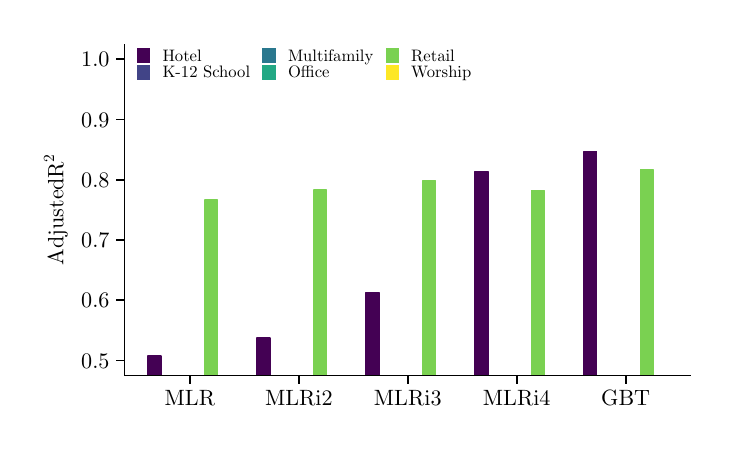
\begin{tikzpicture}[x=1pt,y=1pt]
\definecolor{fillColor}{RGB}{255,255,255}
\path[use as bounding box,fill=fillColor,fill opacity=0.00] (0,0) rectangle (245.72,144.54);
\begin{scope}
\path[clip] (  0.00,  0.00) rectangle (245.72,144.54);
\definecolor{drawColor}{RGB}{255,255,255}
\definecolor{fillColor}{RGB}{255,255,255}

\path[draw=drawColor,line width= 0.6pt,line join=round,line cap=round,fill=fillColor] (  0.00,  0.00) rectangle (245.72,144.54);
\end{scope}
\begin{scope}
\path[clip] ( 34.98, 18.85) rectangle (239.72,138.54);
\definecolor{fillColor}{RGB}{255,255,255}

\path[fill=fillColor] ( 34.98, 18.85) rectangle (239.72,138.54);
\definecolor{drawColor}{RGB}{122,209,81}
\definecolor{fillColor}{RGB}{122,209,81}

\path[draw=drawColor,line width= 0.6pt,line join=round,fill=fillColor] ( 63.99,-84.51) rectangle ( 68.58, 82.18);
\definecolor{drawColor}{RGB}{68,1,84}
\definecolor{fillColor}{RGB}{68,1,84}

\path[draw=drawColor,line width= 0.6pt,line join=round,fill=fillColor] ( 43.51,-84.51) rectangle ( 48.11, 25.82);
\definecolor{drawColor}{RGB}{122,209,81}
\definecolor{fillColor}{RGB}{122,209,81}

\path[draw=drawColor,line width= 0.6pt,line join=round,fill=fillColor] (103.36,-84.51) rectangle (107.95, 85.88);
\definecolor{drawColor}{RGB}{68,1,84}
\definecolor{fillColor}{RGB}{68,1,84}

\path[draw=drawColor,line width= 0.6pt,line join=round,fill=fillColor] ( 82.89,-84.51) rectangle ( 87.48, 32.35);
\definecolor{drawColor}{RGB}{122,209,81}
\definecolor{fillColor}{RGB}{122,209,81}

\path[draw=drawColor,line width= 0.6pt,line join=round,fill=fillColor] (142.73,-84.51) rectangle (147.32, 89.36);
\definecolor{drawColor}{RGB}{68,1,84}
\definecolor{fillColor}{RGB}{68,1,84}

\path[draw=drawColor,line width= 0.6pt,line join=round,fill=fillColor] (122.26,-84.51) rectangle (126.85, 48.88);
\definecolor{drawColor}{RGB}{122,209,81}
\definecolor{fillColor}{RGB}{122,209,81}

\path[draw=drawColor,line width= 0.6pt,line join=round,fill=fillColor] (182.10,-84.51) rectangle (186.70, 85.66);
\definecolor{drawColor}{RGB}{68,1,84}
\definecolor{fillColor}{RGB}{68,1,84}

\path[draw=drawColor,line width= 0.6pt,line join=round,fill=fillColor] (161.63,-84.51) rectangle (166.22, 92.62);
\definecolor{drawColor}{RGB}{122,209,81}
\definecolor{fillColor}{RGB}{122,209,81}

\path[draw=drawColor,line width= 0.6pt,line join=round,fill=fillColor] (221.48,-84.51) rectangle (226.07, 93.28);
\definecolor{drawColor}{RGB}{68,1,84}
\definecolor{fillColor}{RGB}{68,1,84}

\path[draw=drawColor,line width= 0.6pt,line join=round,fill=fillColor] (201.00,-84.51) rectangle (205.60, 99.81);
\end{scope}
\begin{scope}
\path[clip] (  0.00,  0.00) rectangle (245.72,144.54);
\definecolor{drawColor}{RGB}{0,0,0}

\path[draw=drawColor,line width= 0.6pt,line join=round] ( 34.98, 18.85) --
	( 34.98,138.54);
\end{scope}
\begin{scope}
\path[clip] (  0.00,  0.00) rectangle (245.72,144.54);
\definecolor{drawColor}{RGB}{0,0,0}

\node[text=drawColor,anchor=base east,inner sep=0pt, outer sep=0pt, scale=  0.80] at ( 29.58, 21.54) {0.5};

\node[text=drawColor,anchor=base east,inner sep=0pt, outer sep=0pt, scale=  0.80] at ( 29.58, 43.30) {0.6};

\node[text=drawColor,anchor=base east,inner sep=0pt, outer sep=0pt, scale=  0.80] at ( 29.58, 65.06) {0.7};

\node[text=drawColor,anchor=base east,inner sep=0pt, outer sep=0pt, scale=  0.80] at ( 29.58, 86.82) {0.8};

\node[text=drawColor,anchor=base east,inner sep=0pt, outer sep=0pt, scale=  0.80] at ( 29.58,108.58) {0.9};

\node[text=drawColor,anchor=base east,inner sep=0pt, outer sep=0pt, scale=  0.80] at ( 29.58,130.34) {1.0};
\end{scope}
\begin{scope}
\path[clip] (  0.00,  0.00) rectangle (245.72,144.54);
\definecolor{drawColor}{RGB}{0,0,0}

\path[draw=drawColor,line width= 0.6pt,line join=round] ( 31.98, 24.29) --
	( 34.98, 24.29);

\path[draw=drawColor,line width= 0.6pt,line join=round] ( 31.98, 46.06) --
	( 34.98, 46.06);

\path[draw=drawColor,line width= 0.6pt,line join=round] ( 31.98, 67.82) --
	( 34.98, 67.82);

\path[draw=drawColor,line width= 0.6pt,line join=round] ( 31.98, 89.58) --
	( 34.98, 89.58);

\path[draw=drawColor,line width= 0.6pt,line join=round] ( 31.98,111.34) --
	( 34.98,111.34);

\path[draw=drawColor,line width= 0.6pt,line join=round] ( 31.98,133.10) --
	( 34.98,133.10);
\end{scope}
\begin{scope}
\path[clip] (  0.00,  0.00) rectangle (245.72,144.54);
\definecolor{drawColor}{RGB}{0,0,0}

\path[draw=drawColor,line width= 0.6pt,line join=round] ( 34.98, 18.85) --
	(239.72, 18.85);
\end{scope}
\begin{scope}
\path[clip] (  0.00,  0.00) rectangle (245.72,144.54);
\definecolor{drawColor}{RGB}{0,0,0}

\path[draw=drawColor,line width= 0.6pt,line join=round] ( 58.61, 15.85) --
	( 58.61, 18.85);

\path[draw=drawColor,line width= 0.6pt,line join=round] ( 97.98, 15.85) --
	( 97.98, 18.85);

\path[draw=drawColor,line width= 0.6pt,line join=round] (137.35, 15.85) --
	(137.35, 18.85);

\path[draw=drawColor,line width= 0.6pt,line join=round] (176.72, 15.85) --
	(176.72, 18.85);

\path[draw=drawColor,line width= 0.6pt,line join=round] (216.09, 15.85) --
	(216.09, 18.85);
\end{scope}
\begin{scope}
\path[clip] (  0.00,  0.00) rectangle (245.72,144.54);
\definecolor{drawColor}{RGB}{0,0,0}

\node[text=drawColor,anchor=base,inner sep=0pt, outer sep=0pt, scale=  0.80] at ( 58.61,  7.94) {MLR};

\node[text=drawColor,anchor=base,inner sep=0pt, outer sep=0pt, scale=  0.80] at ( 97.98,  7.94) {MLRi2};

\node[text=drawColor,anchor=base,inner sep=0pt, outer sep=0pt, scale=  0.80] at (137.35,  7.94) {MLRi3};

\node[text=drawColor,anchor=base,inner sep=0pt, outer sep=0pt, scale=  0.80] at (176.72,  7.94) {MLRi4};

\node[text=drawColor,anchor=base,inner sep=0pt, outer sep=0pt, scale=  0.80] at (216.09,  7.94) {GBT};
\end{scope}
\begin{scope}
\path[clip] (  0.00,  0.00) rectangle (245.72,144.54);
\definecolor{drawColor}{RGB}{0,0,0}

\node[text=drawColor,rotate= 90.00,anchor=base west,inner sep=0pt, outer sep=0pt, scale=  0.80] at ( 12.86, 58.67) {Adjusted };

\node[text=drawColor,rotate= 90.00,anchor=base west,inner sep=0pt, outer sep=0pt, scale=  0.80] at ( 12.86, 90.04) {R};

\node[text=drawColor,rotate= 90.00,anchor=base west,inner sep=0pt, outer sep=0pt, scale=  0.56] at (  9.59, 95.93) {2};
\end{scope}
\begin{scope}
\path[clip] (  0.00,  0.00) rectangle (245.72,144.54);
\definecolor{fillColor}{RGB}{255,255,255}

\path[fill=fillColor] ( 36.03,124.39) rectangle (161.30,138.54);
\end{scope}
\begin{scope}
\path[clip] (  0.00,  0.00) rectangle (245.72,144.54);
\definecolor{drawColor}{RGB}{68,1,84}
\definecolor{fillColor}{RGB}{68,1,84}

\path[draw=drawColor,line width= 0.6pt,line cap=round,fill=fillColor] ( 39.74,132.17) rectangle ( 44.01,136.83);
\end{scope}
\begin{scope}
\path[clip] (  0.00,  0.00) rectangle (245.72,144.54);
\definecolor{drawColor}{RGB}{65,68,135}
\definecolor{fillColor}{RGB}{65,68,135}

\path[draw=drawColor,line width= 0.6pt,line cap=round,fill=fillColor] ( 39.74,126.10) rectangle ( 44.01,130.75);
\end{scope}
\begin{scope}
\path[clip] (  0.00,  0.00) rectangle (245.72,144.54);
\definecolor{drawColor}{RGB}{42,120,142}
\definecolor{fillColor}{RGB}{42,120,142}

\path[draw=drawColor,line width= 0.6pt,line cap=round,fill=fillColor] ( 85.09,132.17) rectangle ( 89.36,136.83);
\end{scope}
\begin{scope}
\path[clip] (  0.00,  0.00) rectangle (245.72,144.54);
\definecolor{drawColor}{RGB}{34,168,132}
\definecolor{fillColor}{RGB}{34,168,132}

\path[draw=drawColor,line width= 0.6pt,line cap=round,fill=fillColor] ( 85.09,126.10) rectangle ( 89.36,130.75);
\end{scope}
\begin{scope}
\path[clip] (  0.00,  0.00) rectangle (245.72,144.54);
\definecolor{drawColor}{RGB}{122,209,81}
\definecolor{fillColor}{RGB}{122,209,81}

\path[draw=drawColor,line width= 0.6pt,line cap=round,fill=fillColor] (129.61,132.17) rectangle (133.88,136.83);
\end{scope}
\begin{scope}
\path[clip] (  0.00,  0.00) rectangle (245.72,144.54);
\definecolor{drawColor}{RGB}{253,231,37}
\definecolor{fillColor}{RGB}{253,231,37}

\path[draw=drawColor,line width= 0.6pt,line cap=round,fill=fillColor] (129.61,126.10) rectangle (133.88,130.75);
\end{scope}
\begin{scope}
\path[clip] (  0.00,  0.00) rectangle (245.72,144.54);
\definecolor{drawColor}{RGB}{0,0,0}

\node[text=drawColor,anchor=base west,inner sep=0pt, outer sep=0pt, scale=  0.60] at ( 48.72,132.44) {Hotel};
\end{scope}
\begin{scope}
\path[clip] (  0.00,  0.00) rectangle (245.72,144.54);
\definecolor{drawColor}{RGB}{0,0,0}

\node[text=drawColor,anchor=base west,inner sep=0pt, outer sep=0pt, scale=  0.60] at ( 48.72,126.36) {K-12 School};
\end{scope}
\begin{scope}
\path[clip] (  0.00,  0.00) rectangle (245.72,144.54);
\definecolor{drawColor}{RGB}{0,0,0}

\node[text=drawColor,anchor=base west,inner sep=0pt, outer sep=0pt, scale=  0.60] at ( 94.07,132.44) {Multifamily};
\end{scope}
\begin{scope}
\path[clip] (  0.00,  0.00) rectangle (245.72,144.54);
\definecolor{drawColor}{RGB}{0,0,0}

\node[text=drawColor,anchor=base west,inner sep=0pt, outer sep=0pt, scale=  0.60] at ( 94.07,126.36) {Office};
\end{scope}
\begin{scope}
\path[clip] (  0.00,  0.00) rectangle (245.72,144.54);
\definecolor{drawColor}{RGB}{0,0,0}

\node[text=drawColor,anchor=base west,inner sep=0pt, outer sep=0pt, scale=  0.60] at (138.59,132.44) {Retail};
\end{scope}
\begin{scope}
\path[clip] (  0.00,  0.00) rectangle (245.72,144.54);
\definecolor{drawColor}{RGB}{0,0,0}

\node[text=drawColor,anchor=base west,inner sep=0pt, outer sep=0pt, scale=  0.60] at (138.59,126.36) {Worship};
\end{scope}
\end{tikzpicture}
